
\section{Introduction}

\subsection{.NET Framework}

\href{https://www.interviewbit.com/blog/dot-net-framework-architecture/}{.Net Framework Architecture – Detailed Explanation}

The .NET Framework consists of a wide range of components that can be used to build applications for any computer platform.
It includes the core .NET Framework API, which is the set of classes that provides the basic building blocks for applications; several other APIs that are designed to support web technologies; and tools such as Visual Studio.

framework code is largely independent of the language in which it is written.

\begin{figure}[!ht]
  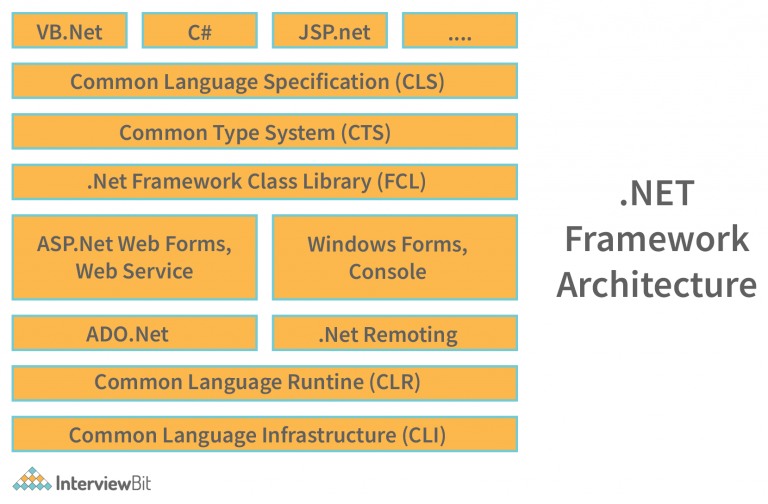
\includegraphics[width=\linewidth]{tools/csharp/images/framework-archi.png}
  \caption{.Net Framework Architecture}
  \label{fig:notnet-archi}
\end{figure}



\subsection{Managed / unmanaged}

In {\bf managed code}, programs run in a managed runtime environment, such as CLR in .NET. The code is compiled into an IL (intermediate language), and it is executed by the runtime, which handles tasks such as memory management, garbage collection, type safety, and exception handling.  

In contrast, the {\bf unmanaged code} operates directly on hardware without using a runtime environment. These are typically low-level programming languages, such as C or C++, which are compiled into native machine code and executed by the CPU itself.

{\bf Risks and Mitigation Strategies for Unmanaged Code}:
\begin{itemize}
    \item Memory management issues
    \item Platform dependencies issues
    \item Security vulnerabilities: Unmanaged code tends to be much more vulnerable to buffer overflows and exploits.  
    \item Concurrency and thread safety: The lack of built-in support for managed concurrency of the unmanaged code can lead to race conditions, deadlocks, and other synchronization issues
    \item Loose pointers: (point to locations with deallocated memory or invalid points in general)
\end{itemize}

\begin{figure}[!ht]
  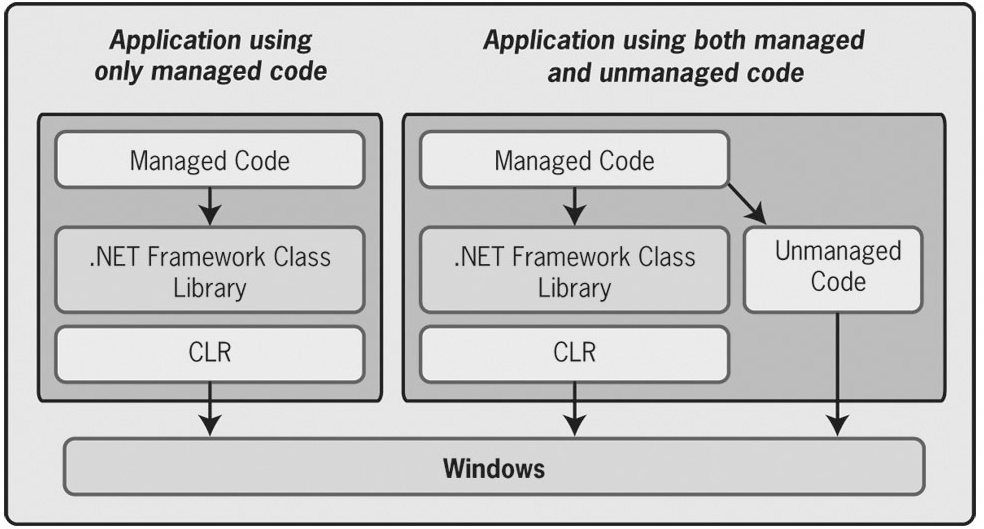
\includegraphics[width=\linewidth]{tools/csharp/images/managed.png}
  \caption{Managed vs Unmanaged}
  \label{fig:notnet-managed}
\end{figure}



\subsection{Platform Invoke (P/Invoke)}
\href{https://learn.microsoft.com/en-us/dotnet/standard/native-interop/pinvoke}{P/Invoke} is a technology that allows you to access structs, callbacks, and functions in unmanaged libraries from your managed code. Most of the P/Invoke API is contained in two namespaces: 
\begin{itemize}
    \item 
        \verb+System+
    \item 
        \verb+System.Runtime.InteropServices+
\end{itemize}

\subsubsection{Invoking unmanaged code from managed code}
\begin{verbatim}
using System;
using System.Runtime.InteropServices;

public partial class Program
{
    // Import user32.dll (containing the function we need) and define
    // the method corresponding to the native function.
    [LibraryImport("user32.dll", StringMarshalling = StringMarshalling.Utf16, SetLastError = true)]
    private static partial int MessageBox(IntPtr hWnd, string lpText, string lpCaption, uint uType);

    public static void Main(string[] args)
    {
        // Invoke the function as a regular managed method.
        MessageBox(IntPtr.Zero, "Command-line message box", "Attention!", 0);
    }
}
\end{verbatim}

\subsubsection{Invoking managed code from unmanaged code}

\subsection{attributes}

These are attributes. An attribute is a declarative tag that is used to convey information to runtime about the behaviors of various elements like classes, methods, structures, enumerators, assemblies etc., in your program. You can add declarative information to a program by using an attribute. A declarative tag is depicted by square (\verb+[ ]+) brackets placed above the element it is used for. 

\subsection{Namespaces}

\href{https://learn.microsoft.com/en-us/dotnet/api/?view=netframework-4.7.2}{.NET API browser}

\begin{itemize}
    \item \verb+System.Runtime.InteropServices+: Provides a wide variety of members that support COM interop and platform invoke services. 
    \item \verb+System.Management.Automation+:  is an extension library for powershell
\end{itemize}